\section{Wellocate as a benchmark and RL environment}
\label{sec:bench}

Our study measures how an agent splits a noisy budget between new candidates and re-tests. We release Wellocate so
others can measure their own agents the same way, and train agents to split the budget better. It runs our campaigns
through a standard reinforcement-learning interface and gives language models the exact prompts ours received. It comes with frozen splits of scrambled GB1 and PhoQ and of generated grid landscapes (Appendix~\ref{app:using}). The environment,
its code, the campaign logs and the analysis behind each number in this paper are at
\url{https://github.com/Xstendyl/wellocate}.

\begin{figure}[tbp]
\centering
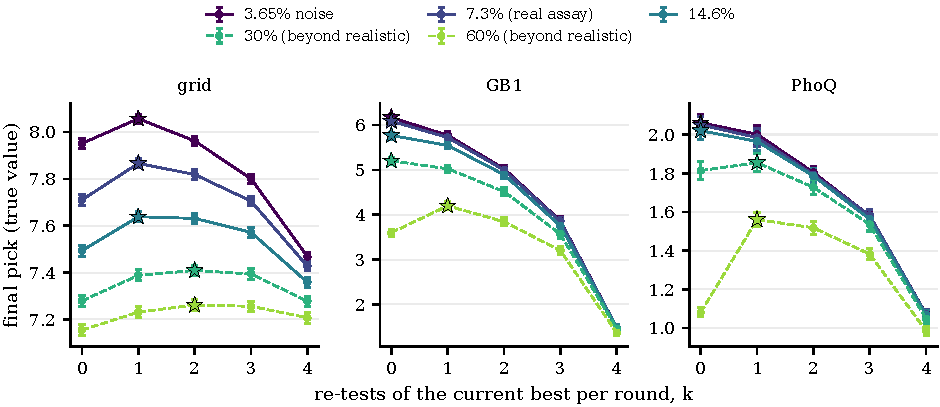
\includegraphics[width=\textwidth]{fig_noise_sweep.pdf}
\caption{The guessing rule's final pick for each number of re-tests per round, with 95\% intervals. Solid curves
cover realistic noise; dashed curves go far beyond it, to show where re-testing starts to pay on the proteins. The star
marks each curve's best setting; where a curve is flat at the top, the star is a near tie.}
\label{fig:noise}
\end{figure}

An environment for this problem is only worth learning in if the right split depends on the situation. If one fixed
rule were best everywhere, there would be nothing to learn. On each landscape,
at five noise levels, we ran the guessing rule at every setting from no re-tests to four a round. We recorded how good its final pick was (Figure~\ref{fig:noise}).

Each curve is one noise level, and its peak, marked with a star, is the best number of re-tests. At the real assay's
noise the grid peaks at one re-test a round. GB1 and PhoQ peak at none, and every re-test added makes the pick worse.
More noise moves the peak: re-testing begins to pay on PhoQ at about \nPhoqTimesLow{} times the assay's noise and on
GB1 only at about \nGbTimesHigh{} times. The reason is how close the best candidates sit. The ten best grid candidates
lie within \nTopSpreadGrid{} noise standard deviations of the best, against \nTopSpreadGb{} on GB1 and \nTopSpreadPq{} on PhoQ. One reading therefore rarely puts protein candidates in the wrong order.

The best fixed rule changes with the landscape and the noise. A good policy has to read the landscape and the noise and set its split from them,
and Wellocate asks a learner to do exactly that. This is also why Section~\ref{sec:res} judges each model against the
best rule for its own landscape and noise.

Last, we asked whether an agent can learn this task inside Wellocate. We trained a small policy from scratch with proximal policy optimisation (PPO), a standard reinforcement-learning method,
only on generated grid landscapes. It never saw a protein or a language model's campaign (Appendix~\ref{app:b11}).
On grid landscapes it had not seen, its final pick beats a policy that orders untried candidates at random by
\nPolRandGrid{} units of true value, and matches the guessing rule. Its lead is not clear on the most rugged generated landscapes. It also works on both proteins, under scrambled and
real names, and stays below the best scripted rule there. In a later check, given the same landscapes, seeds, noise and budget as
each language model's grid campaigns, it picks better than all five models. Replays show what it learned: it builds new
candidates from its best ones and almost never re-tests them. A small learned policy can already beat these models on the
grid, and learning when to confirm is still open.
